\documentclass[10pt]{beamer}

\usetheme[progressbar=frametitle]{metropolis}
\usepackage{appendixnumberbeamer}

\usepackage{booktabs}
\usepackage[scale=2]{ccicons}

\usepackage{pgfplots}
\usepgfplotslibrary{dateplot}
\usepackage{verbatim}
\usepackage{xspace}
\newcommand{\themename}{\textbf{\textsc{metropolis}}\xspace}

\title{Willingness to pay for clean air:Evidence from air purifier markets in China}
\subtitle{Evidence from air purifier markets in China}
 \date{\today}
%\date{}
\author{Hao GENG}
\institute{Department of Economics,CUHK}
 \titlegraphic{\hfill\includegraphics[height=1.5cm]{}}

\begin{document}

\maketitle

\begin{frame}{Table of contents}
  \setbeamertemplate{section in toc}[sections numbered]
  \tableofcontents[hideallsubsections]
\end{frame}

\section{Introduction}

\begin{frame}[fragile]{Why this topic}
.   \begin{itemize}
    \item air pollution is important and severe in developing countries.
    \item a large economic burden of air pollution does not imply that existing environmental regulations are not optimal
    \item to make welfare statements: WTP
\end{itemize}
\end{frame}
\begin{frame}[fragile]{Why estimate air purifier}
    \begin{itemize}
        \item demand for home-use purifiers a main defensive investment for reducing indoor air pollution provides infor as to WTP.
    \end{itemize}
\end{frame}
\begin{frame}{How do we do it?}
    \begin{itemize}
        \item Data:scanner data on market transactions, retail store level, 2006-2012. Pollution data and demographics.
        \item random utility model: Logit&Reg Discontinuity and then BLP.
    \end{itemize}
    
\end{frame}

\begin{frame}{Challenges}
    \begin{itemize}
        \item pollution and price are likely to be endogenous.
        \item spatial regression discontinuity by using Huai River policy in heating supply.
        \item first, product FE and city FE
        \item for product-city level unobserved variables, IV: distance from manufacturing location (import port) to city.
    \end{itemize}
\end{frame}
\begin{frame}{Main Results}
    \begin{itemize}
        \item air pollution is discontinuously higher in cities north.
        \item market share is higher in the north discontinuously.
        \item WTP for removing the amount of PM10 generated by the Huai River policy for five years is USD 190.
        \item MWTP removing 1 ug/m3 for five years is 4.4 usd.
        \item distribution of WTP:BLP. Higher income has higher MWTP.
    \end{itemize}
\end{frame}

\begin{frame}{Contributions}
    \begin{itemize}
        \item we develop a framework to estimate WTP on clean air based on defensive investment
        \item policy implications.
        \item empirical evidence of an important missing piece in the literature of air pollution in developing countries.
    \end{itemize}
\end{frame}

\section{Data}
\begin{frame}{Summary Statistics}
    \begin{columns}[c] 
    \column{9cm}
    \begin{figure}
        \centering
        \includegraphics[height=8cm]{table1}
    \end{figure}
    \column{4cm}
    \begin{itemize}
        \item Air purifier,air pullution,manufacturing/importing location data for each j (IV),demographic info (2005 Census)
        \item air purifier:2006.1-2012.12,81 cities. \ org:product-city-store-y-m after:product-city.
        \item pollution data:
        \item demographics: 
    \end{itemize}
	\end{columns}
\end{frame}

\section{Demand for Air Purifiers}
\begin{frame}{random utility model for differentiated products}
    \begin{itemize}
        \item $u_{ijc}=\beta_{i}x_{jc}+\alpha_{i}p_{jc}+\eta_j+\lambda_c+\xi_{jc}+\epsilon_{ijc}$ (1)
        \item consumer i city c product j
        \item $x_{jc} = x_c\cdot e_j$, where $x_c$:ambient air pollution in this city, $e_j\in [0,1]$ is purifier j's effectiveness to reduce indoor particular matters. 
        \item I think HEPA:high-efficiency particulate arrestance measures $e_j$. 
        \item $x_{jc}$:the improvements in indoor air quality conditional on the purchase of j,$p_jc$,$\eta_j$:product FE,$\lambda_c$ city FE,$\xi_{jc}$:product-city specific demand shock?.
        \item $\epsilon_ijc$: type I extreme value distribution.
    \end{itemize}
\end{frame}

\begin{frame}{4.1 Logit Model}
    \begin{itemize}
        \item $u_{ijc}=\beta_{i}x_{jc}+\alpha_{i}p_{jc}+\eta_j+\lambda_c+\xi_{jc}+\epsilon_{ijc}$ (1)
        \item $\beta_i=\beta$,$\alpha_i=\alpha$
        \item $s_{jc}=\frac{exp(\beta x_{jc}+\alpha p_{jc}+\eta_j+\lambda_c+\xi_{jc})}{\sum_{k=0}^J exp(exp(\beta x_{kc}+\alpha p_{kc}+\eta_k+\lambda_c+\xi_{kc})}$ (2)
        \item outside good:j=0 not to buy.
        \item assume potential buyers are number of households in c, buy either one or zero.\
        $x_{0c}=0$
        \item $lns{0c} = -ln(\sum_{k=0}^J exp(exp(\beta x_{kc}+\alpha p_{kc}+\eta_k+\lambda_c+\xi_{kc}))$ ?
        \item $lns_{jc}-lns_{0c}=\beta x_{jc}+\alpha p_{jc}+\eta_j+\lambda_c+\xi_{jc}$ (3)
        \item $-\beta/\alpha$:marginal utility for clean air/marginal utility from price. Marginal WTP(MWTP).
    \end{itemize}
\end{frame}

\begin{frame}{4.1 Logit Model,Ctd}
    \begin{itemize}
        \item $lns_{jc}-lns_{0c}=\beta x_{jc}+\alpha p_{jc}+\eta_j+\lambda_c+\xi_{jc}$ (3)
        \item $lns_{jc}-lns_{0c}=\beta x_{c}\cdot HEPA_{j}+\alpha_{i}p_{jc}+\eta_j+\lambda_c+\xi_{jc}$ (4) since $x_{jc}=x_c\cdot e_j$,$e_j=HEPA_j$
        \item $-\beta/\alpha$:marginal utility for clean air/marginal utility from price. Marginal WTP(MWTP).
        \item lower bound.
    \end{itemize}
\end{frame}
\subsection{Random-coefficient Logit:BLP}
\begin{frame}{4.2 BLP}
    \begin{itemize}
          \item     standart logit assumes $\beta$ the preference for clean air and price $\alpha$ are indifferent across individuals, thus homogeneous MWTP $-\beta/\alpha$ across individuals.
          \item $\beta_i = \beta_0+\beta_1 y_i +\mu_i$,$\alpha = \alpha_0 +\alpha_{1}y_i+e_i$
          \item $\mu_i\rightarrow N(0,\sigma_\beta),e_i\rightarrow N(0,\sigma_\alpha)$
      \end{itemize}
\end{frame}
\begin{frame}{BLP:Ctd}
    \includegraphics[height=6cm]{ZhangVersusBLP.jpg}
\end{frame}
\begin{frame}{BLP:Ctd}
    \includegraphics[height=\textheight]{ZhangVersusBLP2.jpg}
\end{frame}
\section{Empirical Analysis and Results}
\begin{frame}{5.1 Logit Estimation}
	Endogeneity of air pollution and price motives the author to exploit a regression discontinuity design at the spatial border of Huai River.
	\begin{itemize}
		\item exogenous variation gives more plausibility.
		\item the discontinuous difference in air pollution created by the policy is long-run variation.
%		\item \textsc{Smallcaps}
%		\item \textsc{allsmallcaps}
%		\item ALLCAPS
	\end{itemize}
	They address the endogeneity of prices by combining two approaches.
	\begin{itemize}
	    \item City and product fixed effect.
	    \item For Product-City level unobserved factors:IV .
	\end{itemize}
\end{frame}

\begin{frame}{5.1.1 Empirical Strategy}
	\textbf{First stage on air pollution}
	\begin{itemize}
	    \item local linear reg:$x_c = \gamma North_c +\gamma_1 Lc+ \gamma_2 L_c\cdot North_c+\gamma_3X_c+\epsilon_c$ (7)
	    \item $x_c$: air pollution for city c; $L_c$: the latitude relative to Huai River Boundary; $North_c=1\{L_c>1\}$ dummy for north to the Huai River or not; $X_c$:demographic control.
	\end{itemize}
\end{frame}

\begin{frame}{5.1.1 Empirical Strategy}
	\textbf{Reduced-form on Log Market Share}
	\begin{itemize}
	    \item city-product reg: $lns_{jc}=\rho North_c\cdot HEPA_j+\alpha p_{jc}+(\rho_1 L_c+\rho_2 L_c\cdot North_c)\cdot HEPA_j + \eta_j +\lambda_c+\epsilon_{jc}$ (8)
	    \item $\eta_j$: product FE; $\lambda_c$: City FE; 
	    \item price IV:$distance,distance^2,distance^3$
	    \item \textit{Marginal Willingness to Pay(MWTP):$-\rho/\alpha$}
	    \item WTP for removing the amount of PM10 generated by the Huai River policy for five years is USD 190.
	\end{itemize}
	
	\textbf{Second-Stage on Log Market Share}
	\begin{itemize}
	    \item $lns_{jc}=\beta x_c\cdot HEPA_j+\alpha p_{jc}+(\theta_1 L_c+\theta_2 L_c\cdot North_c)\cdot HEPA_j + \eta_j +\lambda_c+\epsilon_{jc}$ (9)
	    \item using $North_c\cdot HEPA_j$ as the IV for $x_c\cdot HEPA_j$
	    \item using the same IV for price.
	    \item \textit{MWTP: $-\beta/\alpha$}
	    \item MWTP removing 1 ug/m3 for five years is 4.4 usd.
	\end{itemize}
\end{frame}

\begin{frame}{5.1.2 Graphical Analysis}
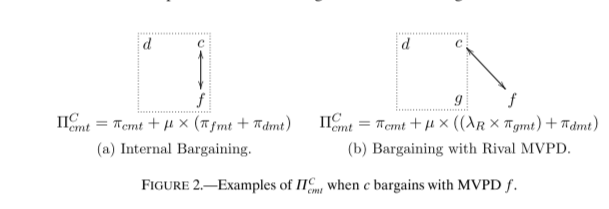
\includegraphics[height=\textheight]{figure2}
\end{frame}

\begin{frame}{5.1.3 Estimation Results using Logit:Stage 1}
    \begin{columns}[c] 
    \column{9cm}
    \begin{figure}
        \centering
        \includegraphics[height=8cm]{table2}
    \end{figure}
    \column{2cm}
    \begin{itemize}
        \item 
    \end{itemize}
	\end{columns}
\end{frame}

\begin{frame}{5.1.3 Estimation Results using Logit:Reduced-Form and Second-Stage}
    \begin{columns}[c] 
    \column{9cm}
    \begin{figure}
        \centering
        \includegraphics[height=8cm]{table3}
    \end{figure}
    \column{4cm}
    \begin{itemize}
        \item Why WTP distincts?
    \end{itemize}
	\end{columns}
\end{frame}

\begin{frame}{5.1.4 Robustness of the Estimates}
    \begin{columns}[c] 
    \column{9cm}
    \begin{figure}
        \centering
        \includegraphics[height=8cm]{table4}
    \end{figure}
    \column{4cm}
    \begin{itemize}
        \item second-stage robustness check
        \item Different bandwidth
        \item Panel A/B:local linear reg/local quadratic reg
    \end{itemize}
	\end{columns}
\end{frame}

\begin{frame}{5.1.5 Potential Confounding Factors to the Estimation}
	\textbf{}
	\begin{itemize}
	    \item Smoothness of running variable in RD design.
	    \item migration of households from north to south.\textbf{Hukou}
	    \item Other policies that use the Huai River Policy. No Chen et al. (2013)
	    \item Subsidy to heating supply in the north,   north households implicitly have higher income.
	    \item availability of HEPA between north and south.
	\end{itemize}
\end{frame}

\section{Random-coefficient Logit Estimation.}

\begin{frame}[fragile]{5.2 Random-coefficient Logit Estimation.}
      \begin{itemize}
          \item     standart logit assumes $\beta$ the preference for clean air and price $\alpha$ are indifferent across individuals, thus homogeneous MWTP $-\beta/\alpha$ across individuals.
          \item $\beta_i = \beta_0+\beta_1 y_i +\mu_i$,$\alpha = \alpha_0 +\alpha_{1}y_i+e_i$
          \item $\mu_i\rightarrow N(0,\sigma_\beta),e_i\rightarrow N(0,\sigma_\alpha)$
      \end{itemize}
\end{frame}


\begin{frame}{5.2.2 Estimation Results}
    \begin{columns}[c] 
    \column{9cm}
    \begin{figure}
        \centering
        \includegraphics[height=8cm]{Figure3}
    \end{figure}
    \column{4cm}
    \begin{itemize}
        \item 
        \item 
        \item 
    \end{itemize}
	\end{columns}
\end{frame}

\begin{frame}{5.2.2 Estimation Results}
    \begin{columns}[c] 
    \column{9cm}
    \begin{figure}
        \centering
        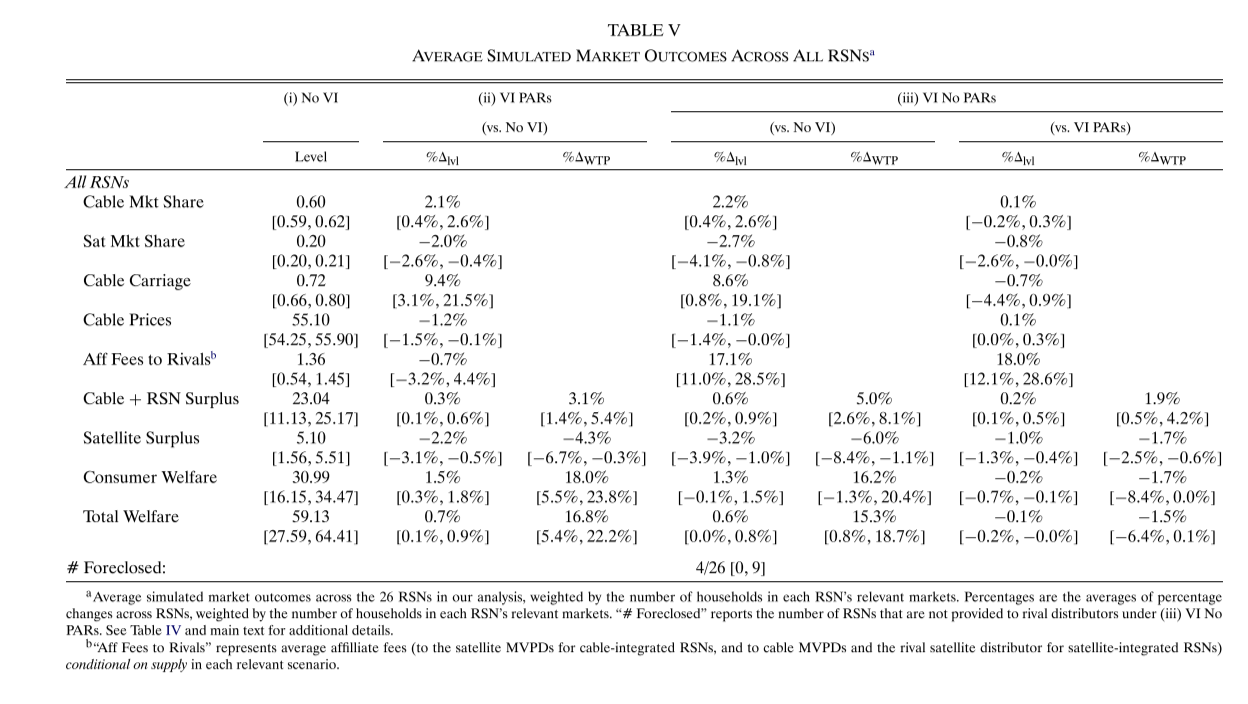
\includegraphics[height=8cm]{table5}
    \end{figure}
    \column{4cm}
    \begin{itemize}
        \item controls for latitude is different between column1,2
        \item MWTP:5.13/5.46 USD slightly larger than logit.
        \item significant $\beta_1$ means positive relationship between $y_i$ and $\beta$. but no significant relationship between $y_i$ and $\alpha$.
        \item coefficient for $\sigma_\alpha$
    \end{itemize}
	\end{columns}
\end{frame}

\begin{frame}{5.2.2 Visual Displaying Estimation Results}
    \begin{columns}[c] 
    \column{9cm}
    \begin{figure}
        \centering
        \includegraphics[height=8cm]{Figure4}
    \end{figure}
    \column{4cm}
    \begin{itemize}
        \item $mwtp_i = -(\hat{\beta_0}+\hat{\beta_1 y_i}+\mu_i)/(\hat{\alpha_0}+\hat{\alpha_1 y_i}+e_i)$
        \item wide dispersion; long right tail
        \item driven by $\beta_1 y_i$ and $e_i$
    \end{itemize}
	\end{columns}
\end{frame}
\begin{frame}{5.2.2 Visual Displaying Estimation Results}
    \begin{columns}[c] 
    \column{9cm}
    \begin{figure}
        \centering
        \includegraphics[height=8cm]{Figure5}
    \end{figure}
    \column{4cm}
    \begin{itemize}
        \item households with income larger than 15000 is dropped in the figure.
        \item increasing with income,mwtp among [0,9] with income among [0,15000].
        \item not suprisingly, the BLP indicates heterogeneity of results: higher-income vs lower-income.
    \end{itemize}
	\end{columns}
\end{frame}
\begin{frame}{Useful tips for programming of BLP}
    \item \url{https://mark-ponder.com/tutorials/static-discrete-choice-models/some-modified-blp-code/}
\end{frame}
\begin{frame}{Font feature test}
  \begin{itemize}
    \item Regular
    \item \textit{Italic}
    \item \textsc{SmallCaps}
    \item \textbf{Bold}
    \item \textbf{\textit{Bold Italic}}
    \item \textbf{\textsc{Bold SmallCaps}}
    \item \texttt{Monospace}
    \item \texttt{\textit{Monospace Italic}}
    \item \texttt{\textbf{Monospace Bold}}
    \item \texttt{\textbf{\textit{Monospace Bold Italic}}}
  \end{itemize}
\end{frame}

\begin{frame}{Lists}
  \begin{columns}[T,onlytextwidth]
    \column{0.33\textwidth}
      Items
      \begin{itemize}
        \item Milk \item Eggs \item Potatos
      \end{itemize}

    \column{0.33\textwidth}
      Enumerations
      \begin{enumerate}
        \item First, \item Second and \item Last.
      \end{enumerate}

    \column{0.33\textwidth}
      Descriptions
      \begin{description}
        \item[PowerPoint] Meeh. \item[Beamer] Yeeeha.
      \end{description}
  \end{columns}
\end{frame}
\begin{frame}{Animation}
  \begin{itemize}[<+- | alert@+>]
    \item \alert<4>{This is\only<4>{ really} important}
    \item Now this
    \item And now this
  \end{itemize}
\end{frame}
\begin{frame}{Figures}
  \begin{figure}
    \newcounter{density}
    \setcounter{density}{20}
    \begin{tikzpicture}
      \def\couleur{alerted text.fg}
      \path[coordinate] (0,0)  coordinate(A)
                  ++( 90:5cm) coordinate(B)
                  ++(0:5cm) coordinate(C)
                  ++(-90:5cm) coordinate(D);
      \draw[fill=\couleur!\thedensity] (A) -- (B) -- (C) --(D) -- cycle;
      \foreach \x in {1,...,40}{%
          \pgfmathsetcounter{density}{\thedensity+20}
          \setcounter{density}{\thedensity}
          \path[coordinate] coordinate(X) at (A){};
          \path[coordinate] (A) -- (B) coordinate[pos=.10](A)
                              -- (C) coordinate[pos=.10](B)
                              -- (D) coordinate[pos=.10](C)
                              -- (X) coordinate[pos=.10](D);
          \draw[fill=\couleur!\thedensity] (A)--(B)--(C)-- (D) -- cycle;
      }
    \end{tikzpicture}
    \caption{Rotated square from
    \href{http://www.texample.net/tikz/examples/rotated-polygons/}{texample.net}.}
  \end{figure}
\end{frame}
\begin{frame}{Tables}
  \begin{table}
    \caption{Largest cities in the world (source: Wikipedia)}
    \begin{tabular}{lr}
      \toprule
      City & Population\\
      \midrule
      Mexico City & 20,116,842\\
      Shanghai & 19,210,000\\
      Peking & 15,796,450\\
      Istanbul & 14,160,467\\
      \bottomrule
    \end{tabular}
  \end{table}
\end{frame}
\begin{frame}{Blocks}
  Three different block environments are pre-defined and may be styled with an
  optional background color.

  \begin{columns}[T,onlytextwidth]
    \column{0.5\textwidth}
      \begin{block}{Default}
        Block content.
      \end{block}

      \begin{alertblock}{Alert}
        Block content.
      \end{alertblock}

      \begin{exampleblock}{Example}
        Block content.
      \end{exampleblock}

    \column{0.5\textwidth}

      \metroset{block=fill}

      \begin{block}{Default}
        Block content.
      \end{block}

      \begin{alertblock}{Alert}
        Block content.
      \end{alertblock}

      \begin{exampleblock}{Example}
        Block content.
      \end{exampleblock}

  \end{columns}
\end{frame}
\begin{frame}{Math}
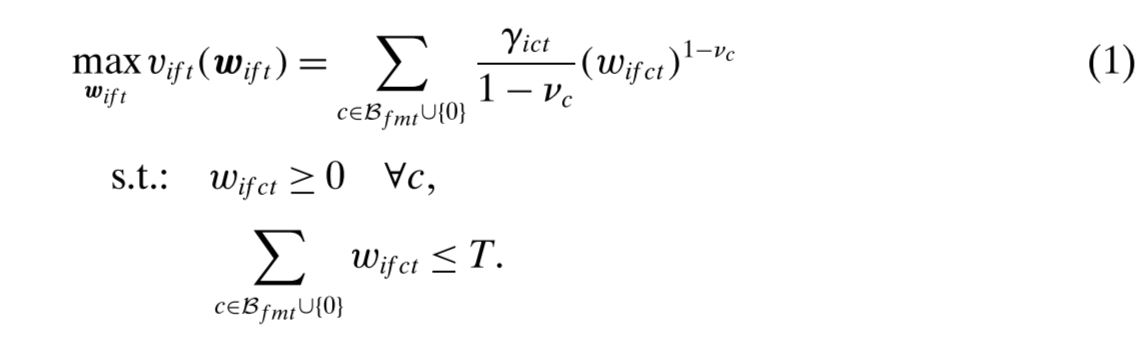
\includegraphics[width=\textwidth]{1}
  \begin{equation*}
    e = \lim_{n\to \infty} \left(1 + \frac{1}{n}\right)^n
  \end{equation*}
\end{frame}
\begin{frame}{Line plots}
  \begin{figure}
    \begin{tikzpicture}
      \begin{axis}[
        mlineplot,
        width=0.9\textwidth,
        height=6cm,
      ]

        \addplot {sin(deg(x))};
        \addplot+[samples=100] {sin(deg(2*x))};

      \end{axis}
    \end{tikzpicture}
  \end{figure}
\end{frame}
\begin{frame}{Bar charts}
  \begin{figure}
    \begin{tikzpicture}
      \begin{axis}[
        mbarplot,
        xlabel={Foo},
        ylabel={Bar},
        width=0.9\textwidth,
        height=6cm,
      ]

      \addplot plot coordinates {(1, 20) (2, 25) (3, 22.4) (4, 12.4)};
      \addplot plot coordinates {(1, 18) (2, 24) (3, 23.5) (4, 13.2)};
      \addplot plot coordinates {(1, 10) (2, 19) (3, 25) (4, 15.2)};

      \legend{lorem, ipsum, dolor}

      \end{axis}
    \end{tikzpicture}
  \end{figure}
\end{frame}
\begin{frame}{Quotes}
  \begin{quote}
    Veni, Vidi, Vici
  \end{quote}
\end{frame}

{%
\setbeamertemplate{frame footer}{My custom footer}
\begin{frame}[fragile]{Frame footer}
    \themename defines a custom beamer template to add a text to the footer. It can be set via
    \begin{verbatim}\setbeamertemplate{frame footer}{My custom footer}\end{verbatim}
\end{frame}
}

\begin{frame}{References}
  Some references to showcase [allowframebreaks] \cite{knuth92,ConcreteMath,Simpson,Er01,greenwade93}
\end{frame}

\section{Conclusion}

\begin{frame}{Summary}

  Get the source of this theme and the demo presentation from

  \begin{center}\url{github.com/matze/mtheme}\end{center}

  The theme \emph{itself} is licensed under a
  \href{http://creativecommons.org/licenses/by-sa/4.0/}{Creative Commons
  Attribution-ShareAlike 4.0 International License}.

  \begin{center}\ccbysa\end{center}

\end{frame}

{\setbeamercolor{palette primary}{fg=black, bg=yellow}
\begin{frame}[standout]
  Questions?
\end{frame}
}
% this is comments.
\begin{comment}
{
    \metroset{titleformat frame=smallcaps}
\begin{frame}{Small caps}
	This frame uses the \texttt{smallcaps} titleformat.

	\begin{alertblock}{Potential Problems}
		Be aware, that not every font supports small caps. If for example you typeset your presentation with pdfTeX and the Computer Modern Sans Serif font, every text in smallcaps will be typeset with the Computer Modern Serif font instead.
	\end{alertblock}
\end{frame}
}

{
\metroset{titleformat frame=allsmallcaps}
\begin{frame}{All small caps}
	This frame uses the \texttt{allsmallcaps} titleformat.

	\begin{alertblock}{Potential problems}
		As this titleformat also uses smallcaps you face the same problems as with the \texttt{smallcaps} titleformat. Additionally this format can cause some other problems. Please refer to the documentation if you consider using it.

		As a rule of thumb: Just use it for plaintext-only titles.
	\end{alertblock}
\end{frame}
}

{
\metroset{titleformat frame=allcaps}
\begin{frame}{All caps}
	This frame uses the \texttt{allcaps} titleformat.

	\begin{alertblock}{Potential Problems}
		This titleformat is not as problematic as the \texttt{allsmallcaps} format, but basically suffers from the same deficiencies. So please have a look at the documentation if you want to use it.
	\end{alertblock}
\end{frame}
}
\end{comment}
\appendix

\begin{frame}[fragile]{Backup slides}
  Sometimes, it is useful to add slides at the end of your presentation to
  refer to during audience questions.

  The best way to do this is to include the \verb|appendixnumberbeamer|
  package in your preamble and call \verb|\appendix| before your backup slides.

  \themename will automatically turn off slide numbering and progress bars for
  slides in the appendix.
\end{frame}

\begin{frame}[allowframebreaks]{References}

  \bibliography{demo}
  \bibliographystyle{abbrv}

\end{frame}

\end{document}

